En el capítulo actual se mostrará la factibilidad que tiene el proyecto de ser realizado.

\section{Factibilidad Técnica}

Identificar necesidades del programa y documentarlas para cumplir objetivos y satisfacer a los usuarios.

Requerimiento de uso del software en computadores:
\begin{table}[h!]
\begin{center}
\begin{tabular}{ | m{0.21\linewidth} | m{0.21\linewidth} | m{0.26\linewidth} | m{0.21\linewidth} |}
\noalign{\hrule height 2pt}
Requisitos mínimos & Windows & macOS & Linux \\ 
\noalign{\hrule height 2pt}

Versión sistema operativo & 
Windows 7 (Service Pack 1+), Windows 10 y Windows 11 & 
High Sierra 10.13+ &
Ubuntu 20.04, Ubuntu 18.04, y CentOS 7
 \\
\hline

Procesador & 
Arquitectura x86 o x64 con soporte de instrucción SSE2 & 
Arquitectura x64 con soporte de instrucción SSE2 para CPU Intel, Apple M1 o superior para CPU Apple & 
Arquitectura x64 con soporte de instrucción SSE2
 \\
\hline

API Gráfico & 
GPU compatible con DirectX versión 10, 11 o 12 & 
GPU Intel, AMD o Apple compatible con Metal &
GPU compatible con OpenGL 3.2+ o Vulkan
 \\
\hline

\end{tabular}
\caption{Requerimientos de operación computadores}
\end{center}
\end{table}

\clearpage

El programa al tener la disponibilidad de poder desarrollar una versión para celulares y derivados que posean el sistema operativo o sean capaz de ejecutar el sistema, se investiga sobre el requerimiento que se necesita en caso de ser ejecutado en alguno de estos dispositivos
\begin{table}[h!]
\begin{center}
\begin{tabular}{ | m{0.30\linewidth} | m{0.30\linewidth} | m{0.3\linewidth} |}
\noalign{\hrule height 2pt}
Requisitos mínimos & Android & iOS \\ 
\noalign{\hrule height 2pt}

Versión sistema operativo & 
Android 5.1 (API 22) & 
iOS 12
 \\
\hline

Procesador & 
ARMV7 compatible con Neon o ARM64 & 
A7 SoC
 \\
\hline

API Gráfico & 
GPU OpenGL ES 2.0 o Vulkan & 
GPU compatible con Metal
 \\
\hline

\end{tabular}
\caption{Requerimientos de operación smartphones}
\end{center}
\end{table}

Debido a que el proyecto tiene enfoque en ser utilizado en el lugar donde reside el usuario, se tomara de base los componentes que poseen los equipos que disponen en la biblioteca, pues se mantiene la idea del contexto en el cual los integrantes de la Universidad no poseen el acceso a el establecimiento, por lo cual se debía realizar el trabajo remoto desde el lugar de residencia. \\

Equipos portátiles:
\begin{itemize}
\item Procesador: Intel i3 8va gen (Por confirmar)
\item GPU: Intel HD Graphics (Por confirmar)
\item Sistema Operativo: Windows 10 (Por confirmar)
\end{itemize}

Utilizando los equipos que se encuentran disponibles en la biblioteca se puede hacer uso de la aplicación correctamente.

\section{Factibilidad Operativa}

El perfil de usuario al que va dirigido principalmente son los alumnos de la Universidad del Bío-Bío, los cuales deseen ocupar o aprender sobre el laboratorio del CIMUBB. Por otra parte, esta puede ser utilizada por cualquier persona.

\subsection{Impacto Positivo}
El impacto positivo de este proyecto es que entrega la posibilidad de poder ocupar virtualmente un laboratorio, sin necesidad de equipamiento, libre de riesgo de romper un equipo costoso.

\begin{comment}
\subsection{Impacto Negativo}
El impacto negativo es la necesidad de capacitar al usuario para el uso de los brazos robóticos, que comandos ejecutan, etc.
\end{comment}

\section{Factibilidad Económica}

Con lo visto en la factibilidad técnica, la Universidad cuenta con ordenadores que pueden ser utilizados, estos no genera gasto pero son contabilizados de igual manera.\\
\clearpage

\begin{table}[h!]
\begin{center}
\begin{tabular}{ | m{0.35\linewidth} | m{0.2\linewidth} |}
\noalign{\hrule height 2pt}
Equipamiento & Costo Por Unidad \\ 
\noalign{\hrule height 2pt}

Equipo Portátil Biblioteca & 
\$314.990
\\
\hline

\end{tabular}
\caption{Costos Equipamiento}
\end{center}
\end{table}

Para los costos del software:
\begin{itemize}
\item Unity: Se puede utilizar la versión gratuita o también la estudiante, posee versiones de pago pero no afecta el resultado.
\item Blender: Es gratuito, posee modelos ya creados de pago y gratuitos que se pueden utilizar.
\item Visual Studio Code: Es gratuito.
\item GitHub: Es gratuito, posee versiones de pago pero para el desarrollo solo influye la mejora de almacenamiento en la nube.
\end{itemize}

Para el desarrollo, al tomar el coste promedio por hora de un Ingeniero Civil Informático en Chile, el cual esta rodeando los \$6.000 por hora. Con este dato se multiplica por las horas de trabajo e investigación, las cuales en al rededor de 13 semanas, tomando en cuenta la ley chilena de no trabajar más de 45 horas a la semana, serian 585 horas en total, lo que daría unos \$3.510.000 \\
Al tomar en cuenta que se esta realizando un proyecto de título, este costo de desarrollo es despreciable. Además de que los equipos ya se encuentran disponibles, estos tampoco generan costo alguno.

\begin{table}[h!]
\begin{center}
\begin{tabular}{ | m{0.35\linewidth} | m{0.2\linewidth} |}
\noalign{\hrule height 2pt}
Variable & Costo  \\ 
\noalign{\hrule height 2pt}

Hardware & \$314.990\\

Software & 
\$0
\\
\hline

Mano de obra & 
\$3.510.000
\\
\hline

Total & 
\$3.824.990
\\
\hline

\end{tabular}
\caption{Resumen de Costos}
\end{center}
\end{table}

Se analiza los gastos que se genera por la necesidad de mantenciones a los brazos robóticos y los gastos de mantener al personal del laboratorio

\begin{table}[h!]
\begin{center}
\begin{tabular}{ | m{0.35\linewidth} | m{0.2\linewidth} |}
\noalign{\hrule height 2pt}
Variable & Costo  Mensual\\ 
\noalign{\hrule height 2pt}

Personal & 
\$1.500.000
\\

Mantención Brazo Robótico & 
\$165.000
\\
\hline

Total & 
\$1.665.000
\\
\hline

\end{tabular}
\caption{Resumen de Gasto Mensual CIMUBB}
\end{center}
\end{table}

Al tener en cuenta la finalidad del proyecto, el cual no busca reemplazar el laboratorio como tal, sino dar una alternativa para poder acceder a la simulación del laboratorio desde el lugar de residencia, se podría reducir las horas de trabajo del personal del laboratorio, el cual trabaja 45 horas a la semana, al contar el mes como cuatro semanas, se obtiene que semanalmente es un gasto de \$375.000. Al ser 45 horas, y contando la semana desde lunes a viernes, el personal trabaja 9 horas diarias, por lo cual diariamente se tiene un gasto de \$75.000. Con esto se analiza que:

\begin{figure}[h]
\centering
    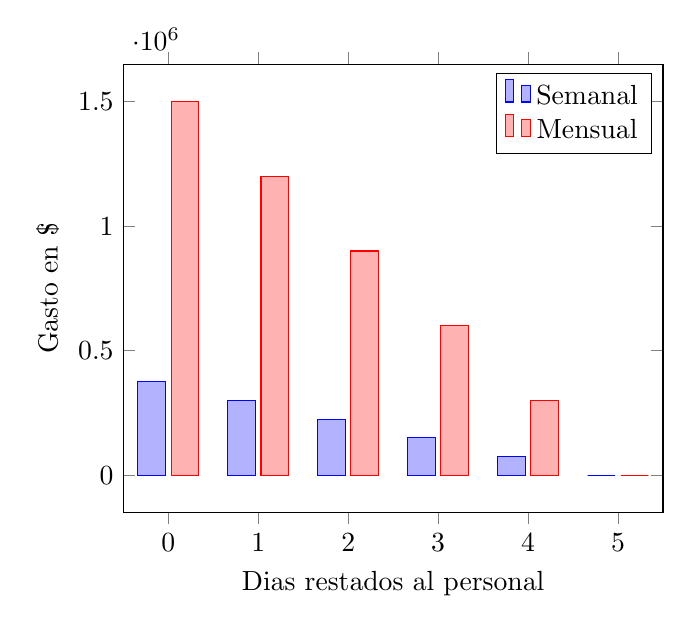
\begin{tikzpicture}
        \begin{axis}[ybar , ylabel={Gasto en \$} , xlabel={Dias restados al personal}]
        \addplot+ [draw = blue] coordinates{
        (0,375000) 
        (1,300000)
        (2,225000)
        (3,150000)
        (4,75000)
        (5,0)
        };
        \addplot+ [draw = red] coordinates{
        (0,1500000) 
        (1,1200000)
        (2,900000)
        (3,600000)
        (4,300000)
        (5,0)
        };
        \legend {Semanal, Mensual}
        \end{axis}
    \end{tikzpicture}
\caption{Análisis gasto Personal CIMUBB}
\label{gasto}
\end{figure}

En la Figura ~\ref{gasto} se logra apreciar la reducción de gasto al reducir los días de trabajo del personal. Sin embargo, para las mantenciones no se pueden reducir, estas son contabilizadas anualmente y son de manera correctiva y no preventiva, siendo esta necesaria por el mal uso de los usuarios y nunca por el desgasto natural.  
\section{Conclusión de la factibilidad}
En cuanto a la factibilidad técnica, la universidad dispone de las herramientas necesarias para el desarrollo y para su uso, se puede llegar a realizar y ocupar sin tener mayores gastos. \\
Por otra parte, al revisar los gastos mensuales, se llega a concluir que la aplicación reduciría un gasto considerable.